\documentclass[10pt,a4paper]{article}
\usepackage[utf8]{inputenc}
\usepackage{algpseudocode}
\usepackage{amsmath}
\usepackage{amsfonts}
\usepackage{amssymb}
\usepackage{graphicx}
\usepackage{hyperref}
\usepackage{listings}
\usepackage{nameref}
\lstset{breaklines}

\begin{document}
\title{Mid-Central US 2015 ICPC Problem Discussion}
\author{Mitch Price\\ Auburn University Programming Team}
\maketitle
\pagebreak
\tableofcontents{}
\pagebreak
\section{ACM Contest Scoring}
\label{acmcontestscoring}
\subsection{Problem Description}

\href{https://open.kattis.com/problems/acm}{View on Kattis}\\
\textbf{Tags:} Implementation\\

In ACM Contest scoring, you are provided with the submission logs for a programming team during an ACM ICPC competition. These logs will consist of a variety of entries of the form: \verb|<submission time> <problem> <status>|, where \verb|<submission>| is the number of minutes into the competition at which the submission was made, \verb|<problem>| is an uppercase letter (A-Z) denoting what problem the submission is for, and \verb|<status>| will be either \verb|right| or \verb|wrong|, indicating whether or not the team got the problem correct.	The submission logs will be sorted by non-decreasing submission time, and will be terminated with a single line containing only the value \verb|-1|.\\

Your program must take these logs and output two numbers: the number of problems successfully solved throughout the contest, and the total penalty time assessed. As a reminder, penalty time is assessed as follows:
\begin{itemize}
	\item No penalty time is assessed for a problem that is not solved during the contest.
	\item For each incorrect submission on a problem that is eventually solved that occurs prior to the given team's first correct submission for that problem, a penalty of 20 minutes is assessed.
	\item When the team correctly solves a problem for the first time, a penalty equal to the submission time of the submission time for the solution is assessed.
	\item The team's total penalty time will be the sum of the penalty times for every problem in the set.
\end{itemize}

\subsection{Algorithm}

This is a fairly straightforward implementation. We simply need to assess the rules as written, which can be done with the following approach:\\

Keep a running total of problems solved and penalty time, initialized to 0. Then, for each submission (in order of increasing submission time):
\begin{itemize}
	\item If the problem has already been solved, do nothing.
	\item Otherwise, if the submission is incorrect, increment the number of incorrect solutions to this problem.
	\item If this problem has not already been solved, but the submission is correct, mark this problem as solved, increment the total number of problems solved, and add the number of incorrect submissions for this problem times 20, plus the submission time to the total penalty time.
\end{itemize}
After doing this for every problem, we just need to output the totals.\\
\hfill\break
\textbf{Time Complexity:} $\mathcal{O}(N)$\\
\textbf{Space Complexity:} $\mathcal{O}(P)$\\
Where \textbf{N} is the number of entries and \textbf{P} is the number of different problems.
\subsection{Implementation}
\lstinputlisting[language=Java]{Solutions/ACM.java}
\pagebreak

\section{Dance Recital}
\label{dancerecital}
\href{https://open.kattis.com/problems/dancerecital}{View on Kattis}\\
\textbf{Tags:} Brute Force, Permutations\\
\subsection{Problem Description}

We are given a list of dance routines, each of which describe a cast of dancers
that will be needed to perform each routine. We want to minimize the number of
times a dancer will perform in back to back routines (called a "quick change").
For example, in the ordering:
\begin{verbatim}
ABC
ABEF
DEF
ABCDE
FGH
\end{verbatim}
There are 6 quick changes (A and B between the 1st and 2nd dances, E and F
between the 2nd and 3rd, and D and E between the 3rd and 4th dances). \\
\hfill\break
However, if we use the ordering:
\begin{verbatim}
ABEF
DEF
ABC
FGH
ABCDE
\end{verbatim}
There are only 2 quick changes (E and F between the 1st and 2nd dances). Given
a list of \textbf{N} routines ($2 \leq N \leq 10$), consisting of dancers
described using only uppercase A-Z letters, determine the minimum number of
quick changes.
\subsection{Algorithm}

Since $10! = 3628800$ is rather tractable, we can brute-force this. However,
in order to make the computation performed at each step as fast as possible,
we will pre-compute the number of quick changes between every pair of dances
and store this ahead of time. Then, each step of the brute force calculation
just requrires us to iterate over the permuted values in order.\\
\hfill\break
Because brute-forcing all permutations of the given values is not the key
part of this excercise, we will rely on our brute-force library to do the
heavy lifting. \\
\hfill\break
\textbf{Time Complexity:} $\mathcal{O}(N! + N \cdot P^2)$\\
\textbf{Space Complexity:} $\mathcal{O}(N(N+P))$\\
Where \textbf{N} is the number of routines ($2 \leq N \leq 10$), and \textbf{P}
 is the number of different dancers ($1 \leq P \leq 26$).
\subsection{Implementation}
\lstinputlisting[language=Java]{Solutions/DanceRecital.java}
\pagebreak

\section{Hidden Password}
\label{hiddenpassword}
\href{https://open.kattis.com/problems/hidden}{View on Kattis}\\
\textbf{Tags:} Strings\\
\subsection{Problem Description}
We are given a password and a message that is supposed to secretly contain the
given password. We must determine if the password is successfully hidden in the
message. In order for this to be the case, the following must hold true:
\begin{itemize}
  \item Denote the password as $P = \{c_{1}, c_{2}, ..., c_{p}\}$.
  \item $c_{1}$ should be the first character in the password to appear in the
  message.
  \item Let $S^{c_{i}}$ denote all characters in the message following the
  character that corresponds to $c_{i}$.
  \item Then the first character in $S^{c_{i}}$ that appears in $P[(i+1) ... p]$
  must equal $c_{i+1}$, for all $ 1 \leq i \leq p-1$.
\end{itemize}
\subsection{Algorithm}
Our algorithm will be a straight-forward implementation of the given check. We
will keep a pointer, \textit{passwordIndex} to which character in the password
we must find next, and iterate over all characters in the message. For each
character \textit{c}, if $c = P[passwordIndex]$, then we increment
\textit{passwordIndex}. Once \textit{passwordIndex} equals $|P|$, we know we
have a match. However, if $c \neq P[passwordIndex]$ and
$\exists \quad i \quad (passwordIndex < i \leq |P|) \quad s.t. \quad c = P[i]$,
then the message and password do not match. Furthermore, if we reach the end of the
message, and $passwordIndex < |P|$, then the message and password do not match.\\
\hfill\break
\textbf{Time Complexity:} $\mathcal{O}(|P| \cdot |S|)$\\
\textbf{Space Complexity:} $\mathcal{O}(|P| + |S|)$\\
Where $|P|$ ($3 \leq |P| \leq 8$) is the length of the password and
$|S|$ ($10 \leq |S| \leq 40$) is the length of the message.
\pagebreak
\subsection{Implementation}
\lstinputlisting[language=Java]{Solutions/HiddenPassword.java}
\pagebreak

\section{Kitchen Measurements}
\label{kitchenmeasurements}
\href{https://open.kattis.com/problems/kitchen}{View on Kattis}\\
\textbf{Tags:} Search, UCS\\
\subsection{Problem Description}

We are given a set of \textit{N} cups $(2 \leq N \leq 5)$ of decreasing
capacities $c_{1}, c_{2}, ..., c_{N}$. The first (and largest) cup is initially
full of water, and all other cups are empty. We are also given a target volume
\textit{V}. Our goal is to end up with exactly \textit{V} units of water in the
first cup, only by pouring water from one cup to another until either the source
cup is empty or the destination cup is full.\\
\hfill\break
If this is impossible, need to say so. Otherwise, we should determine the
minimum amount of liquid that must be poured to achieve the goal.
\subsection{Algorithm}

The solution to this can be derived by performing a Uniform Cost Search, or
Dijkstra's Algorithm. The focus of this exercise will be on determining what
the state space will be, the successor function, and how we will determine
whether or not we are at a goal state. Because performing the search is not the
focus of this, we will be using the search library to perform the acutal search.\\

\textbf{State Space}\\
We will define a state as $\{w_{1}, w_{2}, ... w_{N}\}$, the amount of water in each
cup in the given state. Two states $s_{1} = \{u_{1}, ... u_{N}\}$ and
$s_{2} = \{v_{1}, ... v_{N}\}$ are identical if and only if
$\forall\, i,\, 1 \leq i \leq N,\, v_{i} = u_{i}$.\\

\textbf{Goal State}\\
A given state $s = \{w_{1}, w_{2}, ... w_{N}\}$ is a goal state if and only if
$w_{1} = V$.\\

\textbf{Neighbor Function}\\
We can use the following algorithm to find all neighbors:
\begin{algorithmic}
  \State Let $distance$ be a map of neighbors to distance.
  \For{$src \gets 1$ to $N$}
    \For{$dst \gets 1$ to $N$}
      \If {$src \neq dst$}
        \State $pour \gets \min(w_{src}, c_{dst} - w_{dst})$
        \If {$pour > 0$}
          \State $\{w'_{1}, ... w'_{N}\} \gets \{w_{1}, ... w_{N}\}$
          \State $w'_{src} \gets w'_{src} - pour$
          \State $w'_{dst} \gets w'_{dst} + pour$
          \State $distance (\{w'_{1}, ... w'_{N}\}) \gets pour$
        \EndIf
      \EndIf
    \EndFor
  \EndFor
\end{algorithmic}
With all of the following defined, we can rely on the UCS class in the search
library to find the optimal procedure, if it exists.\\
\hfill\break
\textbf{Time Complexity:} $\mathcal{O}(N^2 \cdot |S| \cdot \log(|S|))$\\
\textbf{Space Complexity:} $\mathcal{O}(|S|)$\\
Where $N$ is the number of cups, and $|S|$ is the number of different states
we can explore. This is loosely bound by ${\displaystyle \prod_{i=1}^{N} c_{i}}$,
but is significantly less than this value in practice.
\subsection{Implementation}
\lstinputlisting[
  language=Java,
  lastline=35
]{Solutions/KitchenMeasurements.java}
\pagebreak
\lstinputlisting[
  language=Java,
  firstline=37
]{Solutions/KitchenMeasurements.java}
\pagebreak

\section{Line Them Up}
\label{linethemup}
\href{https://open.kattis.com/problems/lineup}{View on Kattis}\\
\textbf{Tags:} Strings\\
\subsection{Problem Description}

Given a list of unique, uppercase names, determine if the list is completely
in increasing alphabetical order, completely decreasing alphabetically, or
neither.
\subsection{Algorithm}

We can rely on Java's built-in String.compareTo function to solve this. First,
we will get the result of compareTo between the 2nd and first list elements.

Then, for every other adjacent pair of strings, we can verify that the result
of compareTo is on the same side of 0 as the initial comparison (i.e. they must
be either both positive or both negative). If it isn't, the answer is neither.
If however, the second value is larger than the first for all pairs, we are
ascending. Finally, if the second value is smaller than the first for all pairs,
we are descending.

\hfill\break
\textbf{Time Complexity:} $\mathcal{O}(L \cdot N)$\\
\textbf{Space Complexity:} $\mathcal{O}(L \cdot N)$\\
Where \textit{L} is the length of the longest string.
\pagebreak
\subsection{Implementation}
\lstinputlisting[language=Java]{Solutions/LineThemUp.java}
\pagebreak

\section{Mosaic}
\label{mosaic}
\href{https://open.kattis.com/problems/Mosaic}{View on Kattis}\\
\textbf{Tags:} Bit Manipulation, Search\\
\subsection{Problem Description}

We need to create a mosaic from black and white squares. There are three possible
types of squares:

\begin{itemize}
  \item A square that is completely black.
  \item A square that is completely white.
  \item A half-white, half-black square, divided along the diagonal of the square.
  These can be rotated as necessary.
\end{itemize}

We are given a diagram with the location of every completely black square.
Additionally, each of these completely black squares may contain a number on it:
the number of half-white, half-black squares that are adjacent (up, down, left,
or right) to this square.

An example starting diagram is given in Figure \ref{mosaic:initial-diagram}.

\begin{figure}[h!]
  \centering
  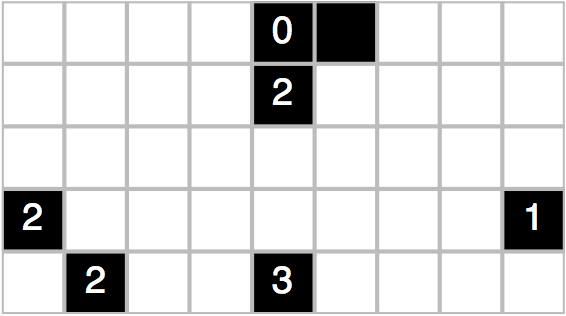
\includegraphics{Images/mosaic-initial.png}
  \caption{Sample Initial Diagram}
  \label{mosaic:initial-diagram}
\end{figure}

Each starting diagram will correspond to exactly 1 completed valid mosaic, which
must satisfy the following criteria:

\begin{itemize}
  \item If a tile in the initial diagram has number on it, that number must
  be realized in the completed mosaic (i.e. if a black square has "2" in the
  initial diagram, that tile must be adjacent to exactly 2 half and half tiles).
  \item Every white shape must be a rectangle (possibly rotated).
\end{itemize}

\begin{figure}[h!]
  \centering
  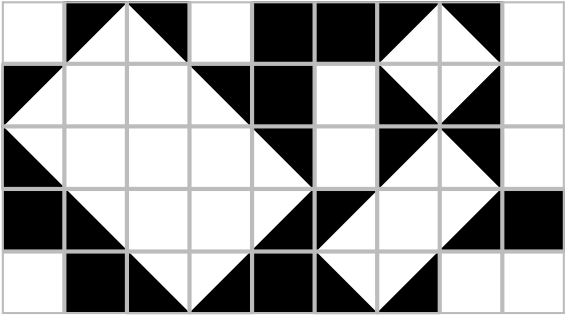
\includegraphics{Images/mosaic-final.png}
  \caption{Completed mosaic for the starting diagram in Figure \ref{mosaic:initial-diagram}}
  \label{mosaic:completed-example}
\end{figure}

\subsection{Algorithm}

The solution for this will be pretty straightforward: we will recursively try
all placements of tiles until we find one that works. However, there is no way
that a naive search will pass the time limit, so we will need to do some pruning. \\

One easy way of pruning the search space while also ensuring that all white areas
in the result will be rectangular is to examine all 2x2 squares containing the
tile you just placed, and ensure that they contain only 180 degree and 90 degree
angles. Additionally, the triangle count contraints for black tiles adjacent to
the tile just placed should also be satisfied.\\

To verify the integrity of a 2x2 square, we can traverse all interior sides of
the selection (they should form a plus-sign), keeping track of whether they
are black or white. At each shared edge, we will examine the color from both
tiles. By doing this in order (either clockwise or counter-clockwise), we can
look for any angles that are not 180 or 90 degrees. Those would have the format
of \verb|<black edge> <n white edges> <black edge>|, where n is either odd
(45, 135, 225, or 315 degrees), or 6 (270 degrees).\\

For example, in Figure \ref{mosaic:example-selection}, we have the edges:
\begin{verbatim}
black, black, white, black, black, black, white, white
\end{verbatim}
As we can see, starting at the second edge there is the subsequence:
\begin{verbatim}
black, white, black
\end{verbatim}
Which, being a 45 degree angle, matches the pattern of an invalid square.\\

\pagebreak

\begin{figure}[h!]
  \centering
  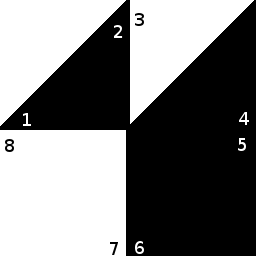
\includegraphics[height=128px]{Images/mosaic-tile-example.png}
  \caption{Example 2x2 selection}
  \label{mosaic:example-selection}
\end{figure}

In order to improve performance even more, we can create a hash function that
will convert any 2x2 square to a unique number and use that to precompute
whether every combination is valid up front, before storing the results in a
boolean array or set.\\

Another option to simplify our logic is to surround the entire puzzle in a region
of black squares at the beginning, which can allow us to get rid of boundary
checks.\\
\hfill\break
\textbf{Time Complexity:} $\mathcal{O}(5^{R \cdot C})$\\
\textbf{Space Complexity:} $\mathcal{O}(R \cdot C)$\\
Where $R$ is the number of rows and $C$ is the number of columns. Due to our
pruning, however, the actual implementation will be much faster than this time
complexity, takes less than a second to process even the largest inputs.
\pagebreak
\subsection{Implementation}
\lstinputlisting[
  lastline=42,
  language=Java
]{Solutions/Mosaic.java}
\pagebreak
\lstinputlisting[
  firstline=44,
  lastline=79,
  language=Java
]{Solutions/Mosaic.java}
\pagebreak
\lstinputlisting[
  firstline=81,
  lastline=128,
  language=Java
]{Solutions/Mosaic.java}
\pagebreak
\lstinputlisting[
  firstline=131,
  lastline=170,
  language=Java
]{Solutions/Mosaic.java}
\pagebreak
\lstinputlisting[
  firstline=172,
  lastline=213,
  language=Java
]{Solutions/Mosaic.java}
\pagebreak
\lstinputlisting[
  firstline=215,
  lastline=247,
  language=Java
]{Solutions/Mosaic.java}
\pagebreak
\lstinputlisting[
  firstline=249,
  language=Java
]{Solutions/Mosaic.java}
\pagebreak

\section{Pyro Tubes}
\label{pyrotubes}
\href{https://open.kattis.com/problems/pyro}{View on Kattis}\\
\textbf{Tags:} Bit Manipulation, Implementation\\
\subsection{Problem Description}
We are given a list of values of brightness to be achieved by illuminating a
selection of tubes. The first tube has a brightness of 1, and each subsequent
tube has double the brightness of the previous tube. For each value, we need to
calculate the number of alternative brightness values. For an alternative value
to be valid, it must satisfy the following:
\begin{itemize}
  \item The alternate value must be greater than the original.
  \item The alternate must be another value in the given list.
  \item The alternate must be achieved by changing no more than 2 tubes from the
  original
\end{itemize}
\subsection{Algorithm}
The key to this is to realize that the tubes simply correspond to bits in the
binary representation of each value. To solve this, we can iterate over all
combinations of 1 or 2 bits in the given range ($2^{0}$ to $2^{17}$, per the
problem statement). We can simply xor the original value with these bits to change
them. If the result is greater than the original, and is in a set containing
all values in the list, we can increment the counter for this value.\\
\hfill\break
\textbf{Time Complexity:} $\mathcal{O}(N \cdot \log^{2}L)$\\
\textbf{Space Complexity:} $\mathcal{O}(N)$\\
Where $N$ is the number of tubes, and $L$ is the largest possible brightness value.
\pagebreak
\subsection{Implementation}
\lstinputlisting[language=Java]{Solutions/PyroTubes.java}
\pagebreak

\section{Square Deal}
\label{squaredeal}
\href{https://open.kattis.com/problems/squaredeal}{View on Kattis}\\
\textbf{Tags:} Brute Force, Geometry\\
\subsection{Problem Description}
Given the width and height of 3 rectangles, can you arrange the rectangles to
form a square?
\subsection{Algorithm}
Because there are exactly 3 rectangles, there are only 2 cases that we need to
consider:
\begin{itemize}
  \item All rectangles can be stacked in a line together (Figure
    \ref{squaredeal:case-1}).
  \item 2 rectangles are stacked together. The other will lie across them
  (Figure \ref{squaredeal:case-2}).
\end{itemize}

\begin{figure}[h!]
  \centering
  \begin{minipage}{0.45\textwidth}
    \centering
    
\includegraphics[width=0.9\textwidth]{Images/squaredeal-case1.png}
    \caption{Case 1}
    \label{squaredeal:case-1}
  \end{minipage}\hfill
  \begin{minipage}{0.45\textwidth}
    \centering
    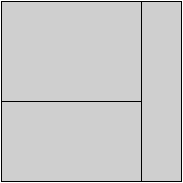
\includegraphics[width=0.9\textwidth]{Images/squaredeal-case2.png}
    \caption{Case 2}
    \label{squaredeal:case-2}
  \end{minipage}
\end{figure}

We can brute force this quite easily. All we need to do is examine all
8 combinations of vertical/horizontal rotations, and then check both cases for
each combination. The first case is one check, and for the second case, we will
need to try all 3 rectangles as the one that isn't stacked with the others.\\

\hfill\break
\textbf{Time Complexity:} $\mathcal{O}(2^{N} \cdot N)$\\
\textbf{Space Complexity:} $\mathcal{O}(N)$\\
Where $N$ is the number of rectangles (3).
\pagebreak
\subsection{Implementation}
\lstinputlisting[
  lastline=47,
  language=Java
]{Solutions/SquareDeal.java}
\pagebreak
\lstinputlisting[
  firstline=49,
  language=Java
]{Solutions/SquareDeal.java}
\pagebreak

\section{The Agglomerator}
\label{theagglomerator}
\href{https://open.kattis.com/problems/agglomerator}{View on Kattis}\\
\textbf{Tags:} Algebra, Geometry\\
\subsection{Problem Description}
We are given the initial positions, initial velocities, and sizes of a
collection of circular droplets in a 2-D grid. When two droplets touch one
another, they will merge into a single droplet. This new droplet's location and
velocity will be the area-weighted average of the 2 initial droplet's locations
and velocities. We need to simulate the movement of the droplets until no more
merges will occur. Luckily, the droplets have the following constraints:

\begin{itemize}
  \item The original droplets do not touch each other.
  \item When a new droplet is formed from a merge, the new droplet will be a
  distance of at least $0.001$ from all other droplets.
  \item Changing the radius of any drop by $\pm 0.001$ will not affect whether
  it collides with any other drop.
  \item All collisions will be at least $0.001$ seconds apart.
  \item No droplets will merge after $t = 10^{9}$ seconds.
\end{itemize}

Given these constraints, determine how many droplets will be left at the end,
and the time of the last merge.\\

\subsection{Algorithm}

To find when (and if) two drops $a$ and $b$ will collide, we can use some basic
algebra. We need to solve for the first time $t$ where the drop's distance is
equal to the sum of their radii:

\begin{equation}
\Bigg | \bigg ( \begin{pmatrix}x_{a} \\ y_{a}\end{pmatrix} + t \cdot
  \begin{pmatrix}v_{ax} \\ v_{ay}\end{pmatrix} \bigg ) - \bigg (
  \begin{pmatrix}x_{a} \\ y_{a}\end{pmatrix} + t \cdot
  \begin{pmatrix}v_{ax} \\ v_{ay}\end{pmatrix} \bigg ) \Bigg |
  =  r_{a} + r_{b}
\end{equation}

To simplify calculatations, let us say
$\begin{pmatrix}x_{a} \\ y_{a}\end{pmatrix} +
\begin{pmatrix}x_{b} \\ y_{b}\end{pmatrix} =
\begin{pmatrix}d_{x} \\ d_{y} \end{pmatrix}$,
$\begin{pmatrix}v_{ax} \\ v_{ay}\end{pmatrix} +
\begin{pmatrix}v_{bx} \\ v_{by}\end{pmatrix} =
\begin{pmatrix}d_{vx} \\ d_{vy}\end{pmatrix}$, and
$r_{a} + r_{b} = s_{r}$.\\

Then, we can reduce the given equality to a quadratic equation:

\begin{equation}
  \big ( d_{vx}^{2} + d_{vy}^{2} \big ) \cdot t^{2} +
  \big ( 2 d_{x} d_{vx} + 2 d_{y} d_{vy} \big ) \cdot t +
  \big ( d_{x}^{2} + d_{y}^{2} - s_{r}^{2} \big ) = 0
\end{equation}

and solve using the quadratic formula
${\big ( -b \pm \sqrt{b^{2} - 4ac} \big ) } / {2a}$, where
$a$ is the coefficient of $t^2$, $b$ is the coefficient of $t$, and $c$ is the
constant term.\\

Because of the constraint that there will be no droplets intersecting at the
start or immediately following a merge, we know that if we look for collisions
at those times, the two solutions for this equation will always have the same
sign. Thus, we can always use the lower solution, which (because $a$ must be
positive) is guaranteed to be the solution in which the root of the determinant
is subtracted. If the determinant or the solution is negative, then the pair
of droplets will not intersect in the future. Otherwise, they will intersect
after the given amount of time.\\

Now that we have a means for finding the time of intersection, we can simulate
the droplets. This can be done as follows:
\hfill\break
\begin{algorithmic}
  \State Let $D$ be a set containing all droplets.
  \State $time \gets 0$
  \While{Another intersection will occur}
    \State Let $a$, $b$ be the droplets that will intersect next, after time $t$.
    \For{$d$ in $D$}
      \State $d \gets advance(d, t)$
    \EndFor
    \State $time \gets time + t$
    \State $D \gets D - a$
    \State $D \gets D - b$
    \State $D \gets D + merge(a, b)$
  \EndWhile
  \State Return $|D|$, $time$
\end{algorithmic}
\hfill\break
Advancing and merging drops simply involves updating the positions of the
droplets as specified in the problem statement.\\
\hfill\break
\textbf{Time Complexity:} $\mathcal{O}(N^{3})$\\
\textbf{Space Complexity:} $\mathcal{O}(N)$\\
Where $N$ is the number of droplets $(2 \leq N \leq 100)$.
\pagebreak
\subsection{Implementation}
\lstinputlisting[
  lastline=45,
  language=Java
  ]{Solutions/Agglomerator.java}
\pagebreak
\lstinputlisting[
  firstline=47,
  lastline=95,
  language=Java
  ]{Solutions/Agglomerator.java}
\pagebreak
\lstinputlisting[
  firstline=97,
  language=Java
  ]{Solutions/Agglomerator.java}
\pagebreak

\section{Word Clouds Revisited}
\label{wordcloudsrevisited}
\href{https://open.kattis.com/problems/wordclouds}{View on Kattis}\\
\textbf{Tags:} Dynamic Programming\\
\subsection{Problem Description}
We are given a list of text boxes, represented with a width and a height. We
need to lay them out within a box of fixed width. An entry can either be placed
horizontally to the right of the previous box (if it fits), or at the far left
end of the next row. The height of each row is the sum of the heights of every
entry in the row. Our goal is to minimize the total height of the word cloud.\\

As it turns out, a greedy solution, as shown in Figure
\ref{wordcloudsrevisited:greedy} may not be the optimal solution, depicted in
Figure \ref{wordcloudsrevisited:optimal}

\begin{figure}[h!]
  \centering
  \begin{minipage}{0.45\textwidth}
    \centering
    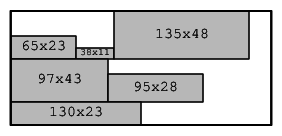
\includegraphics[width=0.9\textwidth]{Images/wordcloudsrevisited-greedy.png}
    \caption{Greedy Strategy}
    \label{wordcloudsrevisited:greedy}
  \end{minipage}
  \hfill
  \begin{minipage}{0.45\textwidth}
    \centering
    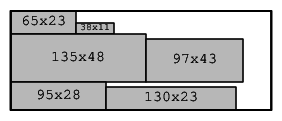
\includegraphics[width=0.9\textwidth]{Images/wordcloudsrevisited-optimal.png}
    \caption{Optimal Solution}
    \label{wordcloudsrevisited:optimal}
  \end{minipage}
\end{figure}

\subsection{Algorithm}

We can make this problem more tractable using dynamic programming. To approach
this problem with that strategy, we need to define two things: an optimal
substructure, and a data structure for memoizing the result.\\

\textbf{Optimal Substructure}\\
An optimal substructure simply represents some way of breaking the problem into
smaller pieces, or some relation that we can use to build upon previous
solutions to smaller portions of the problem. In this case, we can realize that
we only need to track the smallest total height attainable for every possible
width $j$ of the final column after inserting the $ith$ entry. Then, to
calculate the $i+1$th entry's optimal values, we can iterate over all optimal
solutions to the $i$th case and track the results of both inserting in that row
(if possible) or inserting a new row.\\

\pagebreak

\textbf{Data Structure}\\
If we are given $N$ entries and a width of $W$, one option is to store everything
in an $N \cdot (W+1)$ array. To compute the results of the $i$th row, we can
iterate over all columns of the previous row. However, because many columns in
the previous row may not be attainable, we can instead use a map of integers to
optimal values, allowing us to cut down on the average case complexity.
Additionally, because we only need the $i$th row to calculate the $i + 1$th row,
we only need to keep 2 maps, rather than $N$ of them.\\
\hfill\break
Armed with this, we can arrive at the following psuedocode:
\hfill\break
\begin{algorithmic}
  \State Let $best$ be a map of width to the optimal solution for that width.
  \For{Rectangle $r$ in the input}
    \State Let $nextBest$ be a new map of width to the optimal solution.
    \For{$width$, $solution$ in $best$}
      \State $nextBest(r.width) \gets optimal(nextBest(r.width),
        addNewLine(best(width), r))$
      \If{$r.width + width \leq W$}
        \State $newWidth \gets r.width + width$
        \State $nextBest(newWidth) \gets optimal(nextBest(newWidth),
          addSameLine(best(width), r))$
      \EndIf
    \EndFor
    \State $best \gets nextBest$
  \EndFor
  \State Return smallest height in $best$.
\end{algorithmic}
\hfill\break
The optimal solution is whichever minimizes the total height, while $addNewLine$
and $addSameLine$ can be implemented by following the rules of the layout.\\
\hfill\break
\textbf{Time Complexity:} $\mathcal{O}(N \cdot W)$\\
\textbf{Space Complexity:} $\mathcal{O}(W)$\\
Where $N$ is the number of entries $(2 \leq N \leq 5000)$ and $W$ is the width
of the word cloud $(150 \leq W \leq 1000)$.
\pagebreak
\subsection{Implementation}
\lstinputlisting[
  lastline=45,
  language=Java
]{Solutions/WordCloudsRevisited.java}
\pagebreak
\lstinputlisting[
  firstline=47,
  language=Java
]{Solutions/WordCloudsRevisited.java}
\pagebreak

\section{Tags Used}
The following tags appeared throughout the contest:
\begin{itemize}
  \item \textbf{Algebra}: \nameref{theagglomerator}
  \item \textbf{Bit Manipulation}: \nameref{mosaic}, \nameref{pyrotubes}
  \item \textbf{Brute Force}: \nameref{dancerecital}, \nameref{squaredeal}
  \item \textbf{Dynamic Programming}: \nameref{wordcloudsrevisited}
  \item \textbf{Geometry}: \nameref{squaredeal}, \nameref{theagglomerator}
  \item \textbf{Implementation}: \nameref{acmcontestscoring}, \nameref{pyrotubes},
  \item \textbf{Permutations}: \nameref{dancerecital}
  \item \textbf{Search}: \nameref{kitchenmeasurements}, \nameref{mosaic}
  \item \textbf{Strings}: \nameref{hiddenpassword}, \nameref{linethemup}
  \item \textbf{UCS}: \nameref{kitchenmeasurements}
\end{itemize}
\pagebreak
\section{Library Functions Used}
\subsection{Uniform Cost Search (UCS)}
\lstinputlisting[
  lastline=42,
  language=Java
]{Solutions/UCS.java}
\pagebreak
\lstinputlisting[
  firstline=44,
  lastline=81,
  language=Java
]{Solutions/UCS.java}
\pagebreak
\lstinputlisting[
  firstline=83,
  language=Java
]{Solutions/UCS.java}
\pagebreak
\subsection{Permutations}
\lstinputlisting[
  lastline=31,
  language=Java
]{Solutions/Permutations.java}
\pagebreak
\lstinputlisting[
  firstline=33,
  language=Java
]{Solutions/Permutations.java}
\end{document}
